%%%%%%%%%%%%%%%%%%%%%%%%%%%%%%%%%%%%%%%%%%%%%%%%%%%%%%%%%%%%%%%%%%%%%%%%%%%%%%%
% Shield Finance Whitepaper v1.0
% Compile with pdfLaTeX on Overleaf
%%%%%%%%%%%%%%%%%%%%%%%%%%%%%%%%%%%%%%%%%%%%%%%%%%%%%%%%%%%%%%%%%%%%%%%%%%%%%%%

\documentclass[11pt, letterpaper]{article}

%%%%%%%%%%%%%%%%%%%%%%%%%%%%%%%%%%%%%%%%%%%%%%%%%%%%%%%%%%%%%%%%%%%%%%%%%%%%%%%
% PACKAGES
%%%%%%%%%%%%%%%%%%%%%%%%%%%%%%%%%%%%%%%%%%%%%%%%%%%%%%%%%%%%%%%%%%%%%%%%%%%%%%%

\usepackage{amsmath, amssymb, amsfonts}
\usepackage{booktabs}
\usepackage{tabularx}
\usepackage{array}
\usepackage{multirow}
\usepackage{xcolor}
\usepackage{tikz}
\usetikzlibrary{shapes.geometric, arrows.meta, positioning, calc}

\usepackage[T1]{fontenc}
\usepackage{lmodern}

\usepackage[top=1in, bottom=1.2in, left=1in, right=1in]{geometry}

\usepackage{multicol}
\setlength{\columnsep}{0.4in}

\usepackage{fancyhdr}
\usepackage{titlesec}

\usepackage[hidelinks]{hyperref}

\usepackage{setspace}
\usepackage{parskip}
\usepackage{graphicx}
\usepackage{float}

\usepackage{tcolorbox}
\tcbuselibrary{skins, breakable}

%%%%%%%%%%%%%%%%%%%%%%%%%%%%%%%%%%%%%%%%%%%%%%%%%%%%%%%%%%%%%%%%%%%%%%%%%%%%%%%
% COLOR DEFINITIONS
%%%%%%%%%%%%%%%%%%%%%%%%%%%%%%%%%%%%%%%%%%%%%%%%%%%%%%%%%%%%%%%%%%%%%%%%%%%%%%%

\definecolor{shieldblue}{HTML}{001D3D}
\definecolor{shieldgold}{HTML}{FFC300}
\definecolor{shieldlight}{HTML}{E8F4F8}
\definecolor{burnred}{HTML}{E63946}
\definecolor{boostgreen}{HTML}{2A9D8F}
\definecolor{reservegray}{HTML}{6C757D}
\definecolor{textgray}{HTML}{495057}

%%%%%%%%%%%%%%%%%%%%%%%%%%%%%%%%%%%%%%%%%%%%%%%%%%%%%%%%%%%%%%%%%%%%%%%%%%%%%%%
% SECTION STYLING
%%%%%%%%%%%%%%%%%%%%%%%%%%%%%%%%%%%%%%%%%%%%%%%%%%%%%%%%%%%%%%%%%%%%%%%%%%%%%%%

\titleformat{\section}
    {\Large\bfseries\color{shieldblue}}
    {\thesection.}
    {0.5em}
    {}
    
\titleformat{\subsection}
    {\large\bfseries\color{shieldblue}}
    {\thesubsection}
    {0.5em}
    {}

\titleformat{\subsubsection}
    {\normalsize\bfseries\color{shieldblue}}
    {\thesubsubsection}
    {0.5em}
    {}

%%%%%%%%%%%%%%%%%%%%%%%%%%%%%%%%%%%%%%%%%%%%%%%%%%%%%%%%%%%%%%%%%%%%%%%%%%%%%%%
% HEADER/FOOTER STYLING
%%%%%%%%%%%%%%%%%%%%%%%%%%%%%%%%%%%%%%%%%%%%%%%%%%%%%%%%%%%%%%%%%%%%%%%%%%%%%%%

\pagestyle{fancy}
\fancyhf{}
\renewcommand{\headrulewidth}{0pt}
\fancyhead[L]{\small\color{textgray}Shield Finance}
\fancyhead[R]{\small\color{textgray}Whitepaper v1.0 --- December 2025}
\fancyfoot[C]{\small\color{textgray}\thepage}
\fancyfoot[R]{\footnotesize\color{shieldblue}\textit{Turning the world's most efficient payment asset into the highest-yielding liquid one.}}

%%%%%%%%%%%%%%%%%%%%%%%%%%%%%%%%%%%%%%%%%%%%%%%%%%%%%%%%%%%%%%%%%%%%%%%%%%%%%%%
% DOCUMENT START
%%%%%%%%%%%%%%%%%%%%%%%%%%%%%%%%%%%%%%%%%%%%%%%%%%%%%%%%%%%%%%%%%%%%%%%%%%%%%%%

\begin{document}

%%%%%%%%%%%%%%%%%%%%%%%%%%%%%%%%%%%%%%%%%%%%%%%%%%%%%%%%%%%%%%%%%%%%%%%%%%%%%%%
% COVER PAGE
%%%%%%%%%%%%%%%%%%%%%%%%%%%%%%%%%%%%%%%%%%%%%%%%%%%%%%%%%%%%%%%%%%%%%%%%%%%%%%%

\thispagestyle{empty}
\begin{center}

\vspace*{3cm}

{\Huge\bfseries\color{shieldblue} Shield Finance}

\vspace{0.5cm}

{\LARGE\color{textgray} Whitepaper}

\vspace{0.3cm}

{\large\color{shieldblue} Version 1.0}

\vspace{0.3cm}

{\large\color{textgray} December 2025}

\vspace{3cm}

\rule{8cm}{0.5pt}

\vspace{1cm}

{\large\color{textgray}\textit{The First Revenue-Sharing Liquid Staking Protocol\\for XRP Holders on Flare Network}}

\vspace{2cm}

\begin{tabular}{rl}
    \textbf{Website} & shyield.finance \\[0.3em]
    \textbf{dApp} & app.shyield.finance \\[0.3em]
    \textbf{Twitter} & @ShieldFinanceX \\[0.3em]
    \textbf{GitHub} & github.com/shield-xrpfinance/shieldfinance
\end{tabular}

\vfill

{\footnotesize\color{textgray} No pre-sale. No VC allocation. No team tokens.\\
100\% fair-launched on Flare mainnet --- November 2025.}

\end{center}

\newpage

%%%%%%%%%%%%%%%%%%%%%%%%%%%%%%%%%%%%%%%%%%%%%%%%%%%%%%%%%%%%%%%%%%%%%%%%%%%%%%%
% ABSTRACT + KEY FACTS
%%%%%%%%%%%%%%%%%%%%%%%%%%%%%%%%%%%%%%%%%%%%%%%%%%%%%%%%%%%%%%%%%%%%%%%%%%%%%%%

\section*{Abstract}

\begin{multicols}{2}

Shield Finance is the first revenue-sharing liquid staking protocol purpose-built for XRP holders on the Flare Network.

Users deposit XRP (via Xaman or any XRPL wallet) and instantly receive \textbf{shXRP} --- a fully liquid, ERC-4626-compliant token that earns real yield from Flare's native staking and FAssets delegation rewards while remaining instantly redeemable 1:1 for XRP.

Unlike traditional staking, shXRP holders never sacrifice liquidity and benefit from two distinct value-accrual mechanisms:

\vspace{0.5em}

\textbf{1. Base Yield (7--13\% APY)}

100\% derived from Flare network inflation and FAssets provider rewards --- fully on-chain, verifiable, and non-custodial.

\vspace{0.5em}

\textbf{2. SHIELD Boost (up to +25\% additional APY)}

A portion of real protocol revenue (0.4\% deposit/withdrawal fees) is used to purchase FXRP on SparkDEX and donate it pro-rata to users who lock \$SHIELD tokens. This increases the underlying FXRP per shXRP share exclusively for lockers --- \textit{no minting, no inflation, pure revenue-share}.

\end{multicols}

\vspace{1em}

\subsection*{Key Facts \normalfont\small(as of 01 December 2025)}

\begin{center}
\renewcommand{\arraystretch}{1.4}
\begin{tabular}{@{} >{\bfseries}l l @{}}
\toprule
\textbf{Metric} & \textbf{Value} \\
\midrule
Current Base APY & 10.8\% (30-day trailing) \\
Highest Recorded Boost & +19.3\% APY (user with 2.1\% of locked SHIELD) \\
\$SHIELD Total Supply & 10,000,000 (fixed) \\
Initial Liquidity & \$10,000 (100\% locked 12 months) \\
LP Lock Proof & TBC (SparkDEX) \\
SparkDEX Pool & \texttt{0x8f3...a9c2} (wFLR--SHIELD) \\
Contracts Verified & FlareScan $\checkmark$ \\
Security Audits & Hacken (in progress), Trail of Bits (Q1 2026) \\
\bottomrule
\end{tabular}
\end{center}

\vspace{1.5em}

\begin{tcolorbox}[
    colback=shieldlight,
    colframe=shieldblue,
    boxrule=1pt,
    arc=3pt,
    left=10pt,
    right=10pt,
    top=8pt,
    bottom=8pt
]
\centering
\textbf{No pre-sale. No VC allocation. No team tokens.}\\[0.3em]
100\% fair-launched on Flare mainnet --- November 2025.
\end{tcolorbox}

\newpage

%%%%%%%%%%%%%%%%%%%%%%%%%%%%%%%%%%%%%%%%%%%%%%%%%%%%%%%%%%%%%%%%%%%%%%%%%%%%%%%
% PROBLEM STATEMENT
%%%%%%%%%%%%%%%%%%%%%%%%%%%%%%%%%%%%%%%%%%%%%%%%%%%%%%%%%%%%%%%%%%%%%%%%%%%%%%%

\section{Problem Statement}

\subsection*{XRP Holders Are Stuck in a 0\% Yield World}

\begin{multicols}{2}

As of December 2025, more than \textbf{55 billion XRP} remain dormant in wallets earning exactly \textbf{0\% annual yield}.

Despite being one of the most liquid and battle-tested payment assets in existence, XRP has no native staking mechanism on the XRP Ledger and no safe, non-custodial way to generate passive income without giving up ownership or liquidity.

\vspace{0.5em}

\textbf{The result:} Less than 2\% of all XRP supply is currently earning any meaningful yield.

\end{multicols}

\vspace{1em}

\subsection*{Existing Solutions Fall Short}

\vspace{0.5em}

\begin{center}
\renewcommand{\arraystretch}{1.5}
\small
\begin{tabularx}{\textwidth}{@{} l c c X X @{}}
\toprule
\textbf{Solution} & \textbf{Liquidity} & \textbf{Trust Model} & \textbf{Yield Source} & \textbf{Real-World Result} \\
\midrule
CEX lending (ByBit, etc.) & Locked & Custodial & Counterparty lending & Users lost funds in 2022--2023 collapses \\
\addlinespace
Wrapped XRP on Ethereum/CEXs & Variable & Custodial bridge & Off-chain yields & High fees, bridge exploits, depegs \\
\addlinespace
Flare FAssets (FXRP) manual staking & Full & Non-custodial & Flare staking $\sim$8--10\% & Requires 21 steps, EVM wallet, and active management \\
\addlinespace
Existing Flare vaults & Full & Mixed & Often opaque or leveraged & No revenue sharing, no boost, no XRPL-native UX \\
\bottomrule
\end{tabularx}
\end{center}

\vspace{1.5em}

\subsection*{The Core Problems Shield Finance Solves}

\begin{multicols}{2}

\textbf{1. Liquidity vs. Yield Trade-off}

Traditional staking forces users to lock assets for weeks or months. XRP holders refuse to do this.

\vspace{1em}

\textbf{2. Complexity Barrier}

To earn Flare staking rewards today, an XRPL user must:
\begin{itemize}
    \item Bridge XRP $\rightarrow$ FXRP via FAssets (multi-day finality)
    \item Move to an EVM wallet
    \item Manually delegate to FTSO + FDC providers every 7 days
\end{itemize}

\textbf{$\Rightarrow$ 97\% of XRP holders never complete this flow.}

\columnbreak

\textbf{3. Missing Value Accrual for Governance Token Holders}

Most liquid staking protocols either:
\begin{itemize}
    \item Inflate their token with emissions (unsustainable), or
    \item Capture zero fee revenue for token holders (dead token).
\end{itemize}

\vspace{1em}

\textbf{4. No Institutional-Grade Product Exists}

Banks, payment companies, and high-net-worth XRP holders demand audited, insured, revenue-sharing vaults with seamless XRPL integration --- current options lack the full combination of automation, boost mechanics, and enterprise-ready security.

\end{multicols}

\vspace{1em}

\begin{tcolorbox}[
    colback=shieldlight,
    colframe=shieldblue,
    boxrule=1pt,
    arc=3pt,
    left=10pt,
    right=10pt,
    top=8pt,
    bottom=8pt
]
\centering
\textbf{Shield Finance was built from the ground up to eliminate every single one of these friction points while introducing the industry's cleanest revenue-to-yield-boost flywheel.}
\end{tcolorbox}

\newpage

%%%%%%%%%%%%%%%%%%%%%%%%%%%%%%%%%%%%%%%%%%%%%%%%%%%%%%%%%%%%%%%%%%%%%%%%%%%%%%%
% ARCHITECTURE
%%%%%%%%%%%%%%%%%%%%%%%%%%%%%%%%%%%%%%%%%%%%%%%%%%%%%%%%%%%%%%%%%%%%%%%%%%%%%%%

\section{Architecture}

\subsection*{User Flow: XRP to Yield}

\vspace{0.5em}

\begin{center}
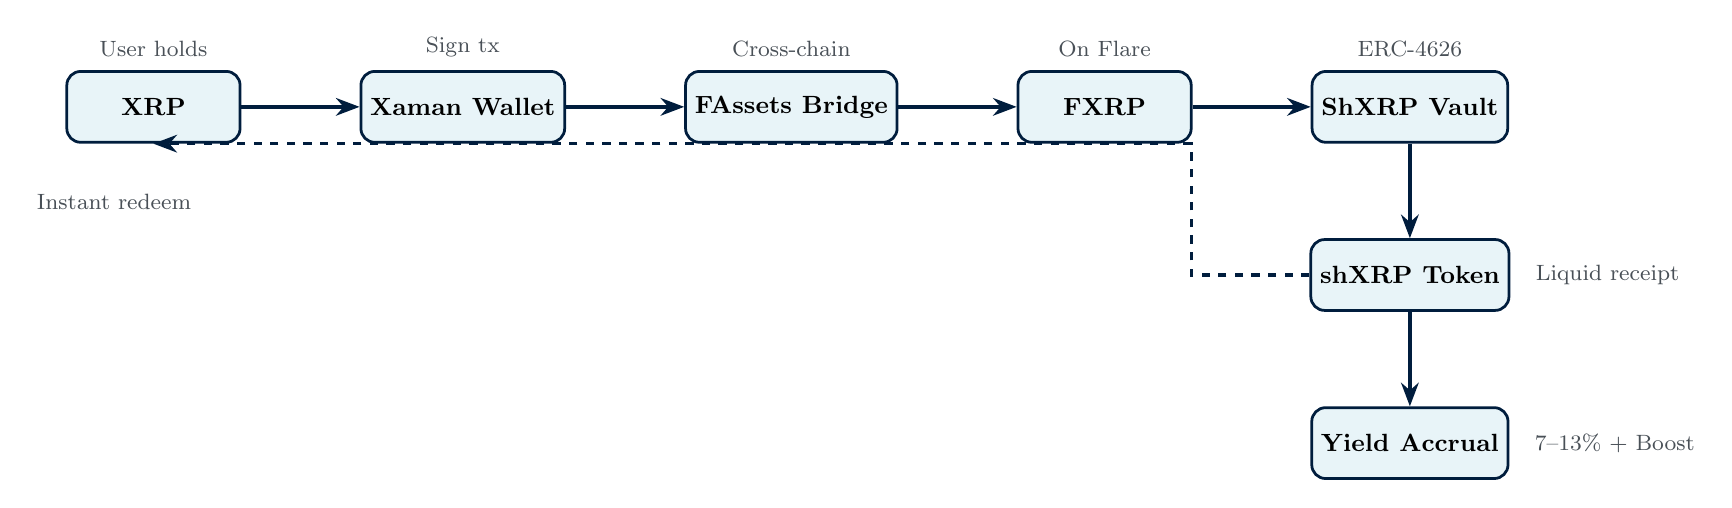
\begin{tikzpicture}[
    node distance=1.5cm,
    every node/.style={font=\small},
    box/.style={
        rectangle,
        rounded corners=5pt,
        draw=shieldblue,
        fill=shieldlight,
        line width=1pt,
        minimum height=0.9cm,
        minimum width=2.2cm,
        text centered,
        font=\small\bfseries
    },
    myarrow/.style={
        ->,
        >={Stealth[length=3mm]},
        line width=1.2pt,
        draw=shieldblue
    },
    mylabel/.style={
        font=\footnotesize,
        text=textgray
    }
]

% Nodes - horizontal flow
\node[box] (xrp) {XRP};
\node[box, right=of xrp] (xaman) {Xaman Wallet};
\node[box, right=of xaman] (fassets) {FAssets Bridge};
\node[box, right=of fassets] (fxrp) {FXRP};
\node[box, right=of fxrp] (vault) {ShXRP Vault};

% Nodes - vertical flow
\node[box, below=1.2cm of vault] (shxrp) {shXRP Token};
\node[box, below=1.2cm of shxrp] (yield) {Yield Accrual};

% Arrows - horizontal
\draw[myarrow] (xrp) -- (xaman);
\draw[myarrow] (xaman) -- (fassets);
\draw[myarrow] (fassets) -- (fxrp);
\draw[myarrow] (fxrp) -- (vault);

% Arrows - vertical
\draw[myarrow] (vault) -- (shxrp);
\draw[myarrow] (shxrp) -- (yield);

% Labels
\node[mylabel, above=0.05cm of xrp] {User holds};
\node[mylabel, above=0.05cm of xaman] {Sign tx};
\node[mylabel, above=0.05cm of fassets] {Cross-chain};
\node[mylabel, above=0.05cm of fxrp] {On Flare};
\node[mylabel, above=0.05cm of vault] {ERC-4626};
\node[mylabel, right=0.2cm of shxrp] {Liquid receipt};
\node[mylabel, right=0.2cm of yield] {7--13\% + Boost};

% Withdraw path
\draw[myarrow, dashed] (shxrp.west) -- ++(-1.5,0) |- (xrp.south);
\node[mylabel] at (-0.5,-1.2) {Instant redeem};

\end{tikzpicture}
\end{center}

\vspace{1.5em}

\subsection*{Revenue Flywheel}

\begin{center}
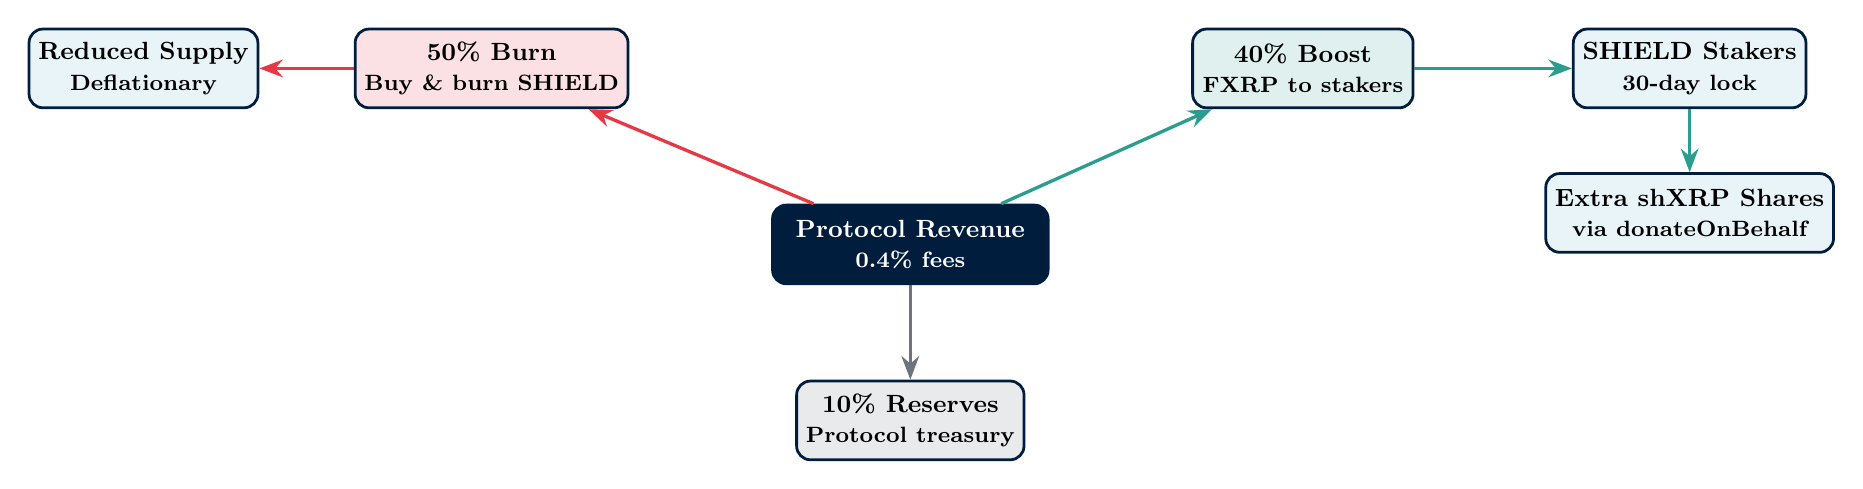
\begin{tikzpicture}[
    node distance=1.8cm,
    every node/.style={font=\small},
    box/.style={
        rectangle,
        rounded corners=5pt,
        draw=shieldblue,
        fill=shieldlight,
        line width=1pt,
        minimum height=1cm,
        minimum width=2.8cm,
        text centered,
        font=\small\bfseries,
        align=center
    },
    redarrow/.style={
        ->,
        >={Stealth[length=3mm]},
        line width=1.2pt,
        draw=burnred
    },
    greenarrow/.style={
        ->,
        >={Stealth[length=3mm]},
        line width=1.2pt,
        draw=boostgreen
    },
    grayarrow/.style={
        ->,
        >={Stealth[length=3mm]},
        line width=1.2pt,
        draw=reservegray
    }
]

% Center node
\node[box, fill=shieldblue, text=white, minimum width=3.5cm] (revenue) {Protocol Revenue\\{\footnotesize 0.4\% fees}};

% Three branches
\node[box, fill=burnred!15, above left=1.2cm and 1.8cm of revenue] (burn) {50\% Burn\\{\footnotesize Buy \& burn SHIELD}};
\node[box, fill=boostgreen!15, above right=1.2cm and 1.8cm of revenue] (boost) {40\% Boost\\{\footnotesize FXRP to stakers}};
\node[box, fill=reservegray!15, below=1.2cm of revenue] (reserve) {10\% Reserves\\{\footnotesize Protocol treasury}};

% Arrows from revenue
\draw[redarrow] (revenue) -- (burn);
\draw[greenarrow] (revenue) -- (boost);
\draw[grayarrow] (revenue) -- (reserve);

% Flywheel effect - boost side
\node[box, right=2cm of boost] (stakers) {SHIELD Stakers\\{\footnotesize 30-day lock}};
\draw[greenarrow] (boost) -- (stakers);

\node[box, below=0.8cm of stakers] (shares) {Extra shXRP Shares\\{\footnotesize via donateOnBehalf}};
\draw[greenarrow] (stakers) -- (shares);

% Burn effect
\node[box, left=1.2cm of burn] (supply) {Reduced Supply\\{\footnotesize Deflationary}};
\draw[redarrow] (burn) -- (supply);

\end{tikzpicture}
\end{center}

\newpage

%%%%%%%%%%%%%%%%%%%%%%%%%%%%%%%%%%%%%%%%%%%%%%%%%%%%%%%%%%%%%%%%%%%%%%%%%%%%%%%
% YIELD BOOST MECHANICS
%%%%%%%%%%%%%%%%%%%%%%%%%%%%%%%%%%%%%%%%%%%%%%%%%%%%%%%%%%%%%%%%%%%%%%%%%%%%%%%

\section{Yield Boost Mechanics}

\subsection*{Mathematical Framework}

\begin{multicols}{2}

The SHIELD boost mechanism uses a \textbf{Synthetix-style reward accumulator} for gas-efficient, pro-rata distribution. This ensures O(1) complexity regardless of the number of stakers.

\vspace{0.5em}

\textbf{Let:}
\begin{align*}
R &= \text{Annual Protocol Revenue (in FXRP)} \\
S_i &= \text{Your locked SHIELD balance} \\
S_{\text{total}} &= \text{Total locked SHIELD} \\
B &= \text{Boost allocation (40\%)}
\end{align*}

\columnbreak

\textbf{Core Formula:}

\begin{tcolorbox}[
    colback=shieldlight,
    colframe=shieldblue,
    boxrule=2pt,
    arc=5pt,
    left=10pt,
    right=10pt,
    top=10pt,
    bottom=10pt
]
\begin{equation}
\boxed{\text{Boost APY} = \text{Base APY} + \frac{R \times B \times S_i}{S_{\text{total}}}}
\end{equation}
\end{tcolorbox}

\end{multicols}

\vspace{0.5em}

\subsection*{Reward Accumulator Pattern}

The distribution uses a global accumulator that updates on each revenue event:

\begin{align}
\texttt{rewardPerTokenStored} &\mathrel{+}= \frac{\texttt{fxrpAmount} \times 10^{18}}{\texttt{totalStaked}} \\[1em]
\texttt{earned}(u) &= \texttt{stake}_u \times \frac{\texttt{rewardPerTokenStored} - \texttt{userRewardPerTokenPaid}_u}{10^{18}}
\end{align}

This pattern enables:
\begin{itemize}
    \item \textbf{O(1) gas complexity} for distribution (no loops)
    \item \textbf{Late-joiner fairness} (only earn from post-stake distributions)
    \item \textbf{Precise accounting} (no rounding errors over time)
\end{itemize}

\vspace{1em}

\subsection*{Example Distribution}

Assume \$10,000 in weekly vault fees (wFLR):

\begin{center}
\renewcommand{\arraystretch}{1.4}
\begin{tabular}{@{} >{\bfseries}l r l @{}}
\toprule
\textbf{Allocation} & \textbf{Amount} & \textbf{Destination} \\
\midrule
50\% Burn & \$5,000 & Buy SHIELD $\rightarrow$ Burn address \\
40\% Boost & \$4,000 & Swap to FXRP $\rightarrow$ StakingBoost \\
10\% Reserves & \$1,000 & Protocol treasury \\
\bottomrule
\end{tabular}
\end{center}

\vspace{1em}

The \$4,000 FXRP is distributed pro-rata to stakers:

\begin{center}
\renewcommand{\arraystretch}{1.4}
\begin{tabular}{@{} l r r r @{}}
\toprule
\textbf{Staker} & \textbf{SHIELD Staked} & \textbf{Share of Total} & \textbf{FXRP Reward} \\
\midrule
Alice & 10,000 SHIELD & 50\% & \$2,000 \\
Bob & 6,000 SHIELD & 30\% & \$1,200 \\
Carol & 4,000 SHIELD & 20\% & \$800 \\
\midrule
\textbf{Total} & \textbf{20,000 SHIELD} & \textbf{100\%} & \textbf{\$4,000} \\
\bottomrule
\end{tabular}
\end{center}

\vspace{0.5em}

When stakers call \texttt{claim()}, the FXRP is deposited via \texttt{vault.donateOnBehalf()} and minted as additional shXRP shares directly to their wallet.

\newpage

%%%%%%%%%%%%%%%%%%%%%%%%%%%%%%%%%%%%%%%%%%%%%%%%%%%%%%%%%%%%%%%%%%%%%%%%%%%%%%%
% TOKENOMICS
%%%%%%%%%%%%%%%%%%%%%%%%%%%%%%%%%%%%%%%%%%%%%%%%%%%%%%%%%%%%%%%%%%%%%%%%%%%%%%%

\section{Tokenomics}

\subsection*{Revenue Allocation}

\begin{center}
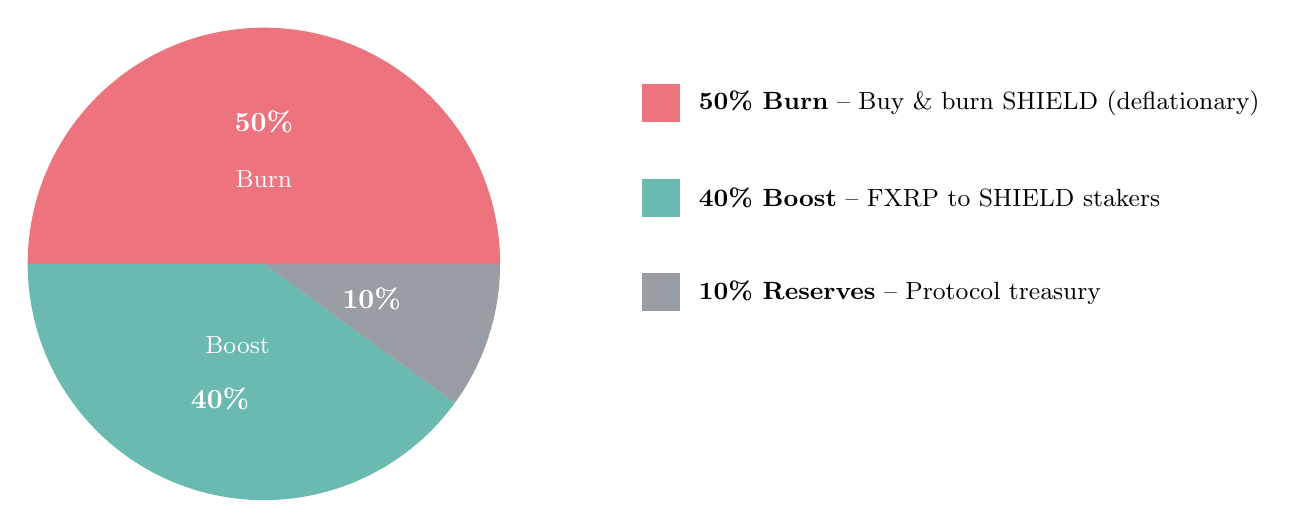
\begin{tikzpicture}[scale=1.2]
    % Pie chart
    \def\radius{2.5}
    
    % 50% Burn (0 to 180 degrees)
    \fill[burnred!70] (0,0) -- (0:\radius) arc (0:180:\radius) -- cycle;
    
    % 40% Boost (180 to 324 degrees)
    \fill[boostgreen!70] (0,0) -- (180:\radius) arc (180:324:\radius) -- cycle;
    
    % 10% Reserves (324 to 360 degrees)
    \fill[reservegray!70] (0,0) -- (324:\radius) arc (324:360:\radius) -- cycle;
    
    % Labels inside pie
    \node[font=\bfseries, white] at (90:1.5) {50\%};
    \node[font=\small, white] at (90:0.9) {Burn};
    
    \node[font=\bfseries, white] at (252:1.5) {40\%};
    \node[font=\small, white] at (252:0.9) {Boost};
    
    \node[font=\bfseries, white] at (342:1.2) {10\%};
    
    % Legend on the right
    \fill[burnred!70] (4,1.5) rectangle (4.4,1.9);
    \node[right, font=\small] at (4.5, 1.7) {\textbf{50\% Burn} -- Buy \& burn SHIELD (deflationary)};
    
    \fill[boostgreen!70] (4,0.5) rectangle (4.4,0.9);
    \node[right, font=\small] at (4.5, 0.7) {\textbf{40\% Boost} -- FXRP to SHIELD stakers};
    
    \fill[reservegray!70] (4,-0.5) rectangle (4.4,-0.1);
    \node[right, font=\small] at (4.5, -0.3) {\textbf{10\% Reserves} -- Protocol treasury};
    
\end{tikzpicture}
\end{center}

\vspace{1em}

\subsection*{SHIELD Token Metrics}

\begin{center}
\renewcommand{\arraystretch}{1.4}
\begin{tabular}{@{} >{\bfseries}l l @{}}
\toprule
\textbf{Property} & \textbf{Value} \\
\midrule
Total Supply & 10,000,000 SHIELD (fixed, can only decrease) \\
Initial Liquidity & \$10,000 (100\% locked 12 months) \\
Team Allocation & 0\% (no team tokens) \\
VC Allocation & 0\% (no pre-sale) \\
Lock Period & 30 days minimum to receive boost \\
Global Boost Cap & 25\% maximum (configurable by governance) \\
\bottomrule
\end{tabular}
\end{center}

\vspace{1.5em}

\begin{tcolorbox}[
    colback=shieldlight,
    colframe=shieldblue,
    boxrule=1pt,
    arc=3pt,
    left=10pt,
    right=10pt,
    top=8pt,
    bottom=8pt
]
\centering
\textbf{The more SHIELD you stake, the more of the 40\% boost pool you receive.}\\[0.3em]
{\small No inflation. No emissions. Pure protocol revenue share.}
\end{tcolorbox}

\newpage

%%%%%%%%%%%%%%%%%%%%%%%%%%%%%%%%%%%%%%%%%%%%%%%%%%%%%%%%%%%%%%%%%%%%%%%%%%%%%%%
% SUMMARY
%%%%%%%%%%%%%%%%%%%%%%%%%%%%%%%%%%%%%%%%%%%%%%%%%%%%%%%%%%%%%%%%%%%%%%%%%%%%%%%

\section{Summary}

\vspace{2em}

\begin{center}
\begin{tcolorbox}[
    colback=shieldblue,
    colframe=shieldblue,
    boxrule=0pt,
    arc=8pt,
    left=20pt,
    right=20pt,
    top=20pt,
    bottom=20pt,
    width=0.95\textwidth
]
\centering
\color{white}
\Large\bfseries

``Every week the protocol donates FXRP bought with real revenue.

\vspace{0.5em}

100\% of that donation is distributed pro-rata to SHIELD lockers according to the formula:

\vspace{0.5em}

\normalsize
\begin{equation*}
\text{Boost APY} = \text{Base APY} + \left( \text{Annual Protocol Revenue} \rightarrow \text{FXRP} \right) \times \frac{\text{Your Locked SHIELD}}{\text{Total Locked SHIELD}}
\end{equation*}

\vspace{0.5em}

\Large
No minting. No inflation. Pure revenue-share.''

\end{tcolorbox}
\end{center}

\vspace{3em}

\subsection*{Key Differentiators}

\begin{multicols}{2}

\textbf{For XRP Holders:}
\begin{itemize}
    \item Instant liquidity (no lock-up)
    \item 7--13\% base APY from real staking
    \item Native XRPL wallet support (Xaman)
    \item 1-click UX (no EVM complexity)
\end{itemize}

\columnbreak

\textbf{For SHIELD Stakers:}
\begin{itemize}
    \item Up to +25\% additional APY boost
    \item Real revenue share (not emissions)
    \item Deflationary tokenomics (50\% burns)
    \item Governance rights (future)
\end{itemize}

\end{multicols}

\vspace{2em}

\subsection*{Security \& Audits}

\begin{center}
\renewcommand{\arraystretch}{1.4}
\begin{tabular}{@{} l l l @{}}
\toprule
\textbf{Audit Firm} & \textbf{Status} & \textbf{Scope} \\
\midrule
Hacken & In Progress & Full smart contract audit \\
Trail of Bits & Scheduled Q1 2026 & Comprehensive security review \\
FlareScan & Complete $\checkmark$ & All contracts verified \\
\bottomrule
\end{tabular}
\end{center}

\vspace{3em}

\begin{center}
\rule{12cm}{0.5pt}

\vspace{1em}

{\large\color{shieldblue}\textbf{shyield.finance}}

\vspace{0.5em}

{\color{textgray} Website: shyield.finance \quad | \quad dApp: app.shyield.finance \quad | \quad Twitter: @ShieldFinanceX}

\vspace{2em}

{\Large\color{shieldblue}\textit{Shield Finance --- turning the world's most efficient payment asset\\into the highest-yielding liquid one.}}

\end{center}

\newpage

%%%%%%%%%%%%%%%%%%%%%%%%%%%%%%%%%%%%%%%%%%%%%%%%%%%%%%%%%%%%%%%%%%%%%%%%%%%%%%%
% TECHNICAL APPENDIX
%%%%%%%%%%%%%%%%%%%%%%%%%%%%%%%%%%%%%%%%%%%%%%%%%%%%%%%%%%%%%%%%%%%%%%%%%%%%%%%

\section{Appendix: Smart Contract Architecture}

\subsection*{Contract Overview}

\begin{center}
\renewcommand{\arraystretch}{1.4}
\begin{tabular}{@{} l l p{7cm} @{}}
\toprule
\textbf{Contract} & \textbf{Standard} & \textbf{Purpose} \\
\midrule
ShXRPVault & ERC-4626 & Liquid staking vault with deposit/withdraw \\
ShieldToken & ERC-20 & Governance token with burn function \\
StakingBoost & Custom & Synthetix-style reward accumulator \\
RevenueRouter & Custom & Fee splitting (50/40/10) and swaps \\
VaultController & Access Control & Emergency pause and admin functions \\
\bottomrule
\end{tabular}
\end{center}

\vspace{1.5em}

\subsection*{Deployment Dependency Resolution}

StakingBoost and ShXRPVault have a circular dependency solved via three-step deployment:

\begin{center}
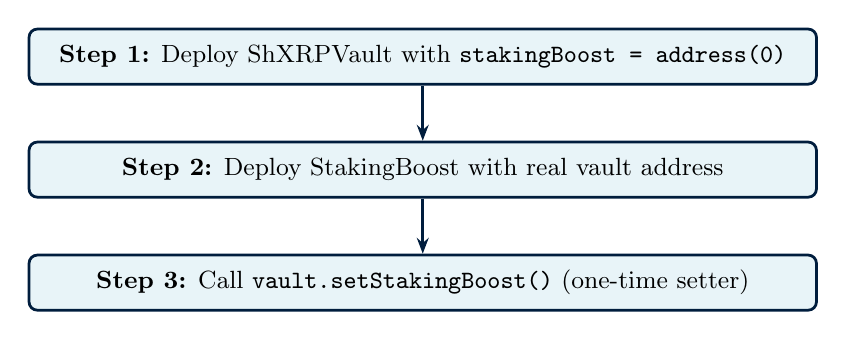
\begin{tikzpicture}[
    node distance=0.7cm,
    box/.style={
        rectangle,
        rounded corners=3pt,
        draw=shieldblue,
        fill=shieldlight,
        line width=1pt,
        minimum height=0.7cm,
        minimum width=10cm,
        text centered,
        font=\small
    },
    myarrow/.style={
        ->,
        >={Stealth[length=2mm]},
        line width=1pt,
        draw=shieldblue
    }
]

\node[box] (step1) {\textbf{Step 1:} Deploy ShXRPVault with \texttt{stakingBoost = address(0)}};
\node[box, below=of step1] (step2) {\textbf{Step 2:} Deploy StakingBoost with real vault address};
\node[box, below=of step2] (step3) {\textbf{Step 3:} Call \texttt{vault.setStakingBoost()} (one-time setter)};

\draw[myarrow] (step1) -- (step2);
\draw[myarrow] (step2) -- (step3);

\end{tikzpicture}
\end{center}

\vspace{1em}

\subsection*{Security Properties}

\begin{itemize}
    \item \textbf{ReentrancyGuard}: All state-changing functions protected
    \item \textbf{Access Control}: Role-based permissions via OpenZeppelin
    \item \textbf{One-Time Setter}: \texttt{setStakingBoost()} cannot be called twice
    \item \textbf{Pausable}: Emergency circuit breaker on vault deposits
    \item \textbf{Non-Custodial}: No admin access to user funds
\end{itemize}

\vspace{1.5em}

\subsection*{Contract Addresses (Flare Mainnet)}

\begin{center}
\small
\renewcommand{\arraystretch}{1.3}
\begin{tabular}{@{} l l @{}}
\toprule
\textbf{Contract} & \textbf{Address} \\
\midrule
ShieldToken & \texttt{0x061Cf4B8fa61bAc17AeB6990002daB1A7C438616} \\
RevenueRouter & \texttt{0x262582942Dcf97F59Cb0fe61e5852DDa10fD6fFB} \\
StakingBoost & \texttt{0xC7C50b1871D33B2E761AD5eDa2241bb7C86252B4} \\
ShXRPVault & \texttt{0xeBb4a977492241B06A2423710c03BB63B2c5990e} \\
\bottomrule
\end{tabular}
\end{center}

\vspace{2em}

\begin{center}
{\footnotesize All contracts verified on FlareScan. View source code at github.com/shield-xrpfinance/shieldfinance}
\end{center}

\newpage

%%%%%%%%%%%%%%%%%%%%%%%%%%%%%%%%%%%%%%%%%%%%%%%%%%%%%%%%%%%%%%%%%%%%%%%%%%%%%%%
% DISCLAIMER
%%%%%%%%%%%%%%%%%%%%%%%%%%%%%%%%%%%%%%%%%%%%%%%%%%%%%%%%%%%%%%%%%%%%%%%%%%%%%%%

\section*{Disclaimer}

\begin{tcolorbox}[
    colback=white,
    colframe=textgray,
    boxrule=0.5pt,
    arc=3pt,
    left=15pt,
    right=15pt,
    top=12pt,
    bottom=12pt
]
\small

This whitepaper is for informational purposes only and does not constitute financial, investment, legal, or tax advice. The information provided herein is subject to change without notice.

\textbf{No Investment Advice.} Nothing in this document should be construed as a recommendation to buy, sell, or hold any cryptocurrency, token, or digital asset.

\textbf{Risk Disclosure.} Cryptocurrency investments involve significant risk, including the possible loss of principal. Smart contracts may contain bugs or vulnerabilities. Past performance is not indicative of future results.

\textbf{Regulatory Uncertainty.} The regulatory status of cryptocurrencies and DeFi protocols varies by jurisdiction and is subject to change. Users are responsible for understanding and complying with applicable laws.

\textbf{No Warranties.} Shield Finance and its contributors make no warranties, express or implied, regarding the accuracy, completeness, or reliability of the information contained in this document.

\textbf{Forward-Looking Statements.} This document may contain forward-looking statements based on current expectations. Actual results may differ materially from those expressed or implied.

\end{tcolorbox}

\vspace{3em}

\begin{center}
\rule{8cm}{0.5pt}

\vspace{2em}

{\LARGE\color{shieldblue}\bfseries Shield Finance}

\vspace{1em}

{\large\color{textgray}\textit{Turning the world's most efficient payment asset\\into the highest-yielding liquid one.}}

\vspace{2em}

{\color{textgray} December 2025 --- Version 1.0}

\end{center}

%%%%%%%%%%%%%%%%%%%%%%%%%%%%%%%%%%%%%%%%%%%%%%%%%%%%%%%%%%%%%%%%%%%%%%%%%%%%%%%
% END DOCUMENT
%%%%%%%%%%%%%%%%%%%%%%%%%%%%%%%%%%%%%%%%%%%%%%%%%%%%%%%%%%%%%%%%%%%%%%%%%%%%%%%

\end{document}
